\documentclass{scrreprt}\usepackage[]{graphicx}\usepackage[]{color}
%% maxwidth is the original width if it is less than linewidth
%% otherwise use linewidth (to make sure the graphics do not exceed the margin)
\makeatletter
\def\maxwidth{ %
  \ifdim\Gin@nat@width>\linewidth
    \linewidth
  \else
    \Gin@nat@width
  \fi
}
\makeatother

\definecolor{fgcolor}{rgb}{0.345, 0.345, 0.345}
\newcommand{\hlnum}[1]{\textcolor[rgb]{0.686,0.059,0.569}{#1}}%
\newcommand{\hlstr}[1]{\textcolor[rgb]{0.192,0.494,0.8}{#1}}%
\newcommand{\hlcom}[1]{\textcolor[rgb]{0.678,0.584,0.686}{\textit{#1}}}%
\newcommand{\hlopt}[1]{\textcolor[rgb]{0,0,0}{#1}}%
\newcommand{\hlstd}[1]{\textcolor[rgb]{0.345,0.345,0.345}{#1}}%
\newcommand{\hlkwa}[1]{\textcolor[rgb]{0.161,0.373,0.58}{\textbf{#1}}}%
\newcommand{\hlkwb}[1]{\textcolor[rgb]{0.69,0.353,0.396}{#1}}%
\newcommand{\hlkwc}[1]{\textcolor[rgb]{0.333,0.667,0.333}{#1}}%
\newcommand{\hlkwd}[1]{\textcolor[rgb]{0.737,0.353,0.396}{\textbf{#1}}}%

\usepackage{framed}
\makeatletter
\newenvironment{kframe}{%
 \def\at@end@of@kframe{}%
 \ifinner\ifhmode%
  \def\at@end@of@kframe{\end{minipage}}%
  \begin{minipage}{\columnwidth}%
 \fi\fi%
 \def\FrameCommand##1{\hskip\@totalleftmargin \hskip-\fboxsep
 \colorbox{shadecolor}{##1}\hskip-\fboxsep
     % There is no \\@totalrightmargin, so:
     \hskip-\linewidth \hskip-\@totalleftmargin \hskip\columnwidth}%
 \MakeFramed {\advance\hsize-\width
   \@totalleftmargin\z@ \linewidth\hsize
   \@setminipage}}%
 {\par\unskip\endMakeFramed%
 \at@end@of@kframe}
\makeatother

\definecolor{shadecolor}{rgb}{.97, .97, .97}
\definecolor{messagecolor}{rgb}{0, 0, 0}
\definecolor{warningcolor}{rgb}{1, 0, 1}
\definecolor{errorcolor}{rgb}{1, 0, 0}
\newenvironment{knitrout}{}{} % an empty environment to be redefined in TeX

\usepackage{alltt}
\title{Flights 1987-2015}
\author{Hugh P}
\IfFileExists{upquote.sty}{\usepackage{upquote}}{}
\begin{document}
\begin{knitrout}
\definecolor{shadecolor}{rgb}{0.969, 0.969, 0.969}\color{fgcolor}\begin{kframe}
\begin{alltt}
\hlstd{START.TIME} \hlkwb{<-} \hlkwd{Sys.time}\hlstd{()}
\hlstd{knitr}\hlopt{::}\hlstd{opts_chunk}\hlopt{$}\hlkwd{set}\hlstd{(}\hlkwc{fig.show} \hlstd{=} \hlstr{'hide'}\hlstd{,}
                      \hlkwc{fig.width} \hlstd{=} \hlnum{8.4}\hlstd{,}
                      \hlkwc{fig.height} \hlstd{=} \hlnum{5}\hlstd{,}
                      \hlkwc{out.width} \hlstd{=} \hlstr{"8.4in"}\hlstd{)}
\end{alltt}
\end{kframe}
\end{knitrout}

\begin{knitrout}
\definecolor{shadecolor}{rgb}{0.969, 0.969, 0.969}\color{fgcolor}\begin{kframe}
\begin{alltt}
\hlkwd{library}\hlstd{(data.table)}
\hlkwd{library}\hlstd{(dplyr)}
\end{alltt}


{\ttfamily\noindent\itshape\color{messagecolor}{\#\# \\\#\# Attaching package: 'dplyr'\\\#\# \\\#\# The following objects are masked from 'package:data.table':\\\#\# \\\#\#\ \ \ \  between, last\\\#\# \\\#\# The following objects are masked from 'package:stats':\\\#\# \\\#\#\ \ \ \  filter, lag\\\#\# \\\#\# The following objects are masked from 'package:base':\\\#\# \\\#\#\ \ \ \  intersect, setdiff, setequal, union}}\begin{alltt}
\hlkwd{library}\hlstd{(magrittr)}
\hlkwd{library}\hlstd{(ggplot2)}
\hlkwd{library}\hlstd{(nycflights13)}  \hlcom{# for airports}
\hlstd{nycflights.airports} \hlkwb{<-} \hlstd{airports}
\hlkwd{library}\hlstd{(fasttime)}
\hlkwd{library}\hlstd{(grattan)}
\end{alltt}


{\ttfamily\noindent\itshape\color{messagecolor}{\#\# Loading required package: devEMF\\\#\# \\\#\# Attaching package: 'grattan'\\\#\# \\\#\# The following object is masked from 'package:datasets':\\\#\# \\\#\#\ \ \ \  Orange}}\end{kframe}
\end{knitrout}

\begin{knitrout}
\definecolor{shadecolor}{rgb}{0.969, 0.969, 0.969}\color{fgcolor}\begin{kframe}
\begin{alltt}
\hlstd{pre2008_flights} \hlkwb{<-}
  \hlkwd{rbindlist}\hlstd{(}\hlkwd{lapply}\hlstd{(}\hlkwd{list.files}\hlstd{(}\hlkwc{path} \hlstd{=} \hlstr{"../flights/1987-2008/"}\hlstd{,}
                    \hlkwc{pattern} \hlstd{=} \hlstr{"csv$"}\hlstd{,}
                    \hlkwc{full.names} \hlstd{=} \hlnum{TRUE}\hlstd{), fread))}

\hlstd{pre2008.names} \hlkwb{<-}
  \hlkwd{names}\hlstd{(pre2008_flights)}

\hlstd{read_and_report} \hlkwb{<-}
  \hlkwa{function}\hlstd{(}\hlkwc{filename}\hlstd{)\{}
    \hlstd{year} \hlkwb{<-} \hlkwd{gsub}\hlstd{(}\hlstr{"^.*(2[0-9]\{3\}).\{3,4\}csv$"}\hlstd{,} \hlstr{"\textbackslash{}\textbackslash{}1"}\hlstd{, filename)}
    \hlkwa{if}\hlstd{(}\hlkwd{grepl}\hlstd{(}\hlstr{"1.csv"}\hlstd{, filename,} \hlkwc{fixed} \hlstd{=} \hlnum{TRUE}\hlstd{))}
      \hlkwd{cat}\hlstd{(year)}
    \hlkwd{fread}\hlstd{(filename,} \hlkwc{select} \hlstd{= pre2008.names,} \hlkwc{showProgress} \hlstd{=} \hlnum{FALSE}\hlstd{)}
  \hlstd{\}}

\hlkwd{gc}\hlstd{(}\hlnum{1}\hlstd{,}\hlnum{1}\hlstd{)}
\hlstd{post2008_flights} \hlkwb{<-}
  \hlkwd{rbindlist}\hlstd{(}\hlkwd{lapply}\hlstd{(}\hlkwd{list.files}\hlstd{(}\hlkwc{path} \hlstd{=} \hlstr{"../flights"}\hlstd{,} \hlkwc{recursive} \hlstd{=} \hlnum{TRUE}\hlstd{,} \hlkwc{pattern} \hlstd{=} \hlstr{"2[0-9]\{3\}.\{3,4\}csv$"}\hlstd{,}
                              \hlkwc{full.names} \hlstd{=} \hlnum{TRUE}\hlstd{),}
                   \hlstd{read_and_report))}

\hlstd{flights} \hlkwb{<-} \hlkwd{rbindlist}\hlstd{(}\hlkwd{list}\hlstd{(pre2008_flights, post2008_flights),} \hlkwc{use.names} \hlstd{=} \hlnum{TRUE}\hlstd{)}
\hlstd{readr}\hlopt{::}\hlkwd{write_csv}\hlstd{(flights,} \hlkwc{path} \hlstd{=} \hlstr{"../1987-2015-On-Time-Performance.csv"}\hlstd{)}
\end{alltt}
\end{kframe}
\end{knitrout}

\begin{knitrout}
\definecolor{shadecolor}{rgb}{0.969, 0.969, 0.969}\color{fgcolor}\begin{kframe}
\begin{alltt}
\hlkwd{Sys.time}\hlstd{()}
\end{alltt}
\begin{verbatim}
## [1] "2016-01-05 22:31:02 AEDT"
\end{verbatim}
\begin{alltt}
\hlstd{flights} \hlkwb{<-} \hlkwd{fread}\hlstd{(}\hlstr{"../1987-2015-On-Time-Performance.csv"}\hlstd{)}
\end{alltt}
\begin{verbatim}
## 
Read 0.0% of 165931626 rows
Read 0.5% of 165931626 rows
Read 1.0% of 165931626 rows
Read 1.5% of 165931626 rows
Read 2.0% of 165931626 rows
Read 2.6% of 165931626 rows
Read 3.1% of 165931626 rows
Read 3.6% of 165931626 rows
Read 4.1% of 165931626 rows
Read 4.6% of 165931626 rows
Read 5.1% of 165931626 rows
Read 5.7% of 165931626 rows
Read 6.2% of 165931626 rows
Read 6.7% of 165931626 rows
Read 7.2% of 165931626 rows
Read 7.7% of 165931626 rows
Read 8.3% of 165931626 rows
Read 8.8% of 165931626 rows
Read 9.3% of 165931626 rows
Read 9.8% of 165931626 rows
Read 10.3% of 165931626 rows
Read 10.8% of 165931626 rows
Read 11.4% of 165931626 rows
Read 11.9% of 165931626 rows
Read 12.4% of 165931626 rows
Read 12.9% of 165931626 rows
Read 13.4% of 165931626 rows
Read 14.0% of 165931626 rows
Read 14.5% of 165931626 rows
Read 15.0% of 165931626 rows
Read 15.5% of 165931626 rows
Read 16.0% of 165931626 rows
Read 16.5% of 165931626 rows
Read 17.1% of 165931626 rows
Read 17.6% of 165931626 rows
Read 18.1% of 165931626 rows
Read 18.6% of 165931626 rows
Read 19.1% of 165931626 rows
Read 19.7% of 165931626 rows
Read 20.2% of 165931626 rows
Read 20.7% of 165931626 rows
Read 21.2% of 165931626 rows
Read 21.7% of 165931626 rows
Read 22.2% of 165931626 rows
Read 22.8% of 165931626 rows
Read 23.3% of 165931626 rows
Read 23.8% of 165931626 rows
Read 24.3% of 165931626 rows
Read 24.8% of 165931626 rows
Read 25.3% of 165931626 rows
Read 25.9% of 165931626 rows
Read 26.4% of 165931626 rows
Read 26.9% of 165931626 rows
Read 27.4% of 165931626 rows
Read 27.9% of 165931626 rows
Read 28.5% of 165931626 rows
Read 29.0% of 165931626 rows
Read 29.5% of 165931626 rows
Read 30.0% of 165931626 rows
Read 30.5% of 165931626 rows
Read 31.0% of 165931626 rows
Read 31.6% of 165931626 rows
Read 32.1% of 165931626 rows
Read 32.6% of 165931626 rows
Read 33.1% of 165931626 rows
Read 33.6% of 165931626 rows
Read 34.2% of 165931626 rows
Read 34.7% of 165931626 rows
Read 35.2% of 165931626 rows
Read 35.7% of 165931626 rows
Read 36.2% of 165931626 rows
Read 36.7% of 165931626 rows
Read 37.3% of 165931626 rows
Read 37.8% of 165931626 rows
Read 38.3% of 165931626 rows
Read 38.8% of 165931626 rows
Read 39.3% of 165931626 rows
Read 39.8% of 165931626 rows
Read 40.4% of 165931626 rows
Read 40.9% of 165931626 rows
Read 41.4% of 165931626 rows
Read 41.9% of 165931626 rows
Read 42.4% of 165931626 rows
Read 43.0% of 165931626 rows
Read 43.5% of 165931626 rows
Read 44.0% of 165931626 rows
Read 44.5% of 165931626 rows
Read 45.0% of 165931626 rows
Read 45.5% of 165931626 rows
Read 46.1% of 165931626 rows
Read 46.6% of 165931626 rows
Read 47.1% of 165931626 rows
Read 47.6% of 165931626 rows
Read 48.1% of 165931626 rows
Read 48.7% of 165931626 rows
Read 49.2% of 165931626 rows
Read 49.7% of 165931626 rows
Read 50.2% of 165931626 rows
Read 50.7% of 165931626 rows
Read 51.3% of 165931626 rows
Read 51.8% of 165931626 rows
Read 52.3% of 165931626 rows
Read 52.8% of 165931626 rows
Read 53.4% of 165931626 rows
Read 53.9% of 165931626 rows
Read 54.4% of 165931626 rows
Read 54.9% of 165931626 rows
Read 55.5% of 165931626 rows
Read 56.0% of 165931626 rows
Read 56.5% of 165931626 rows
Read 57.0% of 165931626 rows
Read 57.5% of 165931626 rows
Read 58.1% of 165931626 rows
Read 58.6% of 165931626 rows
Read 59.1% of 165931626 rows
Read 59.6% of 165931626 rows
Read 60.2% of 165931626 rows
Read 60.7% of 165931626 rows
Read 61.2% of 165931626 rows
Read 61.7% of 165931626 rows
Read 62.3% of 165931626 rows
Read 62.8% of 165931626 rows
Read 63.3% of 165931626 rows
Read 63.8% of 165931626 rows
Read 64.4% of 165931626 rows
Read 64.9% of 165931626 rows
Read 65.4% of 165931626 rows
Read 65.9% of 165931626 rows
Read 66.5% of 165931626 rows
Read 67.0% of 165931626 rows
Read 67.5% of 165931626 rows
Read 68.0% of 165931626 rows
Read 68.6% of 165931626 rows
Read 69.1% of 165931626 rows
Read 69.6% of 165931626 rows
Read 70.1% of 165931626 rows
Read 70.6% of 165931626 rows
Read 71.2% of 165931626 rows
Read 71.7% of 165931626 rows
Read 72.2% of 165931626 rows
Read 72.7% of 165931626 rows
Read 73.2% of 165931626 rows
Read 73.7% of 165931626 rows
Read 74.2% of 165931626 rows
Read 74.7% of 165931626 rows
Read 75.3% of 165931626 rows
Read 75.8% of 165931626 rows
Read 76.3% of 165931626 rows
Read 76.8% of 165931626 rows
Read 77.3% of 165931626 rows
Read 77.8% of 165931626 rows
Read 78.3% of 165931626 rows
Read 78.8% of 165931626 rows
Read 79.4% of 165931626 rows
Read 79.9% of 165931626 rows
Read 80.4% of 165931626 rows
Read 80.9% of 165931626 rows
Read 81.4% of 165931626 rows
Read 81.9% of 165931626 rows
Read 82.4% of 165931626 rows
Read 82.9% of 165931626 rows
Read 83.5% of 165931626 rows
Read 84.0% of 165931626 rows
Read 84.5% of 165931626 rows
Read 85.0% of 165931626 rows
Read 85.5% of 165931626 rows
Read 86.0% of 165931626 rows
Read 86.5% of 165931626 rows
Read 87.0% of 165931626 rows
Read 87.5% of 165931626 rows
Read 88.1% of 165931626 rows
Read 88.6% of 165931626 rows
Read 89.1% of 165931626 rows
Read 89.6% of 165931626 rows
Read 90.1% of 165931626 rows
Read 90.6% of 165931626 rows
Read 91.1% of 165931626 rows
Read 91.6% of 165931626 rows
Read 92.2% of 165931626 rows
Read 92.7% of 165931626 rows
Read 93.2% of 165931626 rows
Read 93.7% of 165931626 rows
Read 94.2% of 165931626 rows
Read 94.7% of 165931626 rows
Read 95.2% of 165931626 rows
Read 95.7% of 165931626 rows
Read 96.3% of 165931626 rows
Read 96.8% of 165931626 rows
Read 97.3% of 165931626 rows
Read 97.8% of 165931626 rows
Read 98.3% of 165931626 rows
Read 98.8% of 165931626 rows
Read 99.3% of 165931626 rows
Read 99.8% of 165931626 rows
Read 165931626 rows and 29 (of 29) columns from 15.111 GB file in 00:03:50
\end{verbatim}
\begin{alltt}
\hlcom{# flights <- readRDS("../1987-2015-On-Time-Performance.rds")}
\end{alltt}
\end{kframe}
\end{knitrout}

\begin{knitrout}
\definecolor{shadecolor}{rgb}{0.969, 0.969, 0.969}\color{fgcolor}\begin{kframe}
\begin{alltt}
\hlstd{flightsSanFran} \hlkwb{<-} \hlstd{flights[Origin} \hlopt \hlkwd{c}\hlstd{(}\hlstr{"SFO"}\hlstd{,} \hlstr{"OAK"}\hlstd{)} \hlopt{|} \hlstd{Dest} \hlopt \hlkwd{c}\hlstd{(}\hlstr{"SFO"}\hlstd{,} \hlstr{"OAK"}\hlstd{)]}
\hlstd{sample.frac} \hlkwb{=} \hlnum{0.2}
\hlstd{sample.weight.int} \hlkwb{=} \hlkwd{as.integer}\hlstd{(}\hlkwd{round}\hlstd{(}\hlnum{1}\hlopt{/}\hlstd{sample.frac))}
\hlstd{flights} \hlkwb{<-} \hlstd{flights[}\hlkwd{sample}\hlstd{(.N, .N} \hlopt{*} \hlstd{sample.frac)]}
\end{alltt}
\end{kframe}
\end{knitrout}

\begin{knitrout}
\definecolor{shadecolor}{rgb}{0.969, 0.969, 0.969}\color{fgcolor}\begin{kframe}
\begin{alltt}
\hlcom{# First we want a time for each flight. This is more difficult that it might seem.}
\hlcom{# We need to concatenate the Year, Month, and DayofMonth fields, but we also need }
\hlcom{# to take into account the various time zones of the airports in the database.}
\hlstd{integer.cols} \hlkwb{<-} \hlkwd{grep}\hlstd{(}\hlstr{"Time$"}\hlstd{,} \hlkwd{names}\hlstd{(flights))}

\hlkwd{Sys.time}\hlstd{()}
\end{alltt}
\begin{verbatim}
## [1] "2016-01-05 22:35:40 AEDT"
\end{verbatim}
\begin{alltt}
\hlkwa{for} \hlstd{(j} \hlkwa{in} \hlstd{integer.cols)\{}
  \hlkwd{set}\hlstd{(flights,} \hlkwc{j} \hlstd{= j,} \hlkwc{value} \hlstd{=} \hlkwd{as.integer}\hlstd{(flights[[j]]))}
\hlstd{\}}
\hlkwd{Sys.time}\hlstd{()}
\end{alltt}
\begin{verbatim}
## [1] "2016-01-05 22:35:40 AEDT"
\end{verbatim}
\begin{alltt}
\hlcom{# See stackoverflow: links and comments under my question}
\hlstd{create_DepDateTime} \hlkwb{<-} \hlkwa{function}\hlstd{(}\hlkwc{DT}\hlstd{)\{}
  \hlkwd{setkey}\hlstd{(DT, Year, Month, DayofMonth, DepTime)}
  \hlstd{unique_dates} \hlkwb{<-} \hlkwd{unique}\hlstd{(DT[,}\hlkwd{list}\hlstd{(Year, Month, DayofMonth, DepTime)])}
  \hlstd{unique_dates[,DepDateTime} \hlkwb{:=} \hlkwd{fastPOSIXct}\hlstd{(}\hlkwd{sprintf}\hlstd{(}\hlstr{"%d-%02d-%02d %s"}\hlstd{, Year, Month, DayofMonth,}
                                                   \hlkwd{sub}\hlstd{(}\hlstr{"([0-9]\{2\})([0-9]\{2\})"}\hlstd{,} \hlstr{"\textbackslash{}\textbackslash{}1:\textbackslash{}\textbackslash{}2:00"}\hlstd{,} \hlkwd{sprintf}\hlstd{(}\hlstr{"%04d"}\hlstd{, DepTime),}
                                                       \hlkwc{perl} \hlstd{=} \hlnum{TRUE}\hlstd{)),}
                                           \hlkwc{tz} \hlstd{=} \hlstr{"GMT"}\hlstd{)]}
  \hlstd{DT[unique_dates]}
\hlstd{\}}

\hlstd{create_ArrDateTime} \hlkwb{<-} \hlkwa{function}\hlstd{(}\hlkwc{DT}\hlstd{)\{}
  \hlkwd{setkey}\hlstd{(DT, Year, Month, DayofMonth, ArrTime)}
  \hlstd{unique_dates} \hlkwb{<-} \hlkwd{unique}\hlstd{(DT[,}\hlkwd{list}\hlstd{(Year, Month, DayofMonth, ArrTime)])}
  \hlstd{unique_dates[,ArrDateTime} \hlkwb{:=} \hlkwd{fastPOSIXct}\hlstd{(}\hlkwd{sprintf}\hlstd{(}\hlstr{"%d-%02d-%02d %s"}\hlstd{, Year, Month, DayofMonth,}
                                                   \hlkwd{sub}\hlstd{(}\hlstr{"([0-9]\{2\})([0-9]\{2\})"}\hlstd{,} \hlstr{"\textbackslash{}\textbackslash{}1:\textbackslash{}\textbackslash{}2:00"}\hlstd{,} \hlkwd{sprintf}\hlstd{(}\hlstr{"%04d"}\hlstd{, ArrTime),}
                                                       \hlkwc{perl} \hlstd{=} \hlnum{TRUE}\hlstd{)),}
                                           \hlkwc{tz} \hlstd{=} \hlstr{"GMT"}\hlstd{)]}
  \hlstd{DT[unique_dates]}
\hlstd{\}}
\hlstd{flights} \hlkwb{<-} \hlkwd{create_DepDateTime}\hlstd{(flights)}
\hlstd{flights} \hlkwb{<-} \hlkwd{create_ArrDateTime}\hlstd{(flights)}
\hlcom{#flights[,`:=`(Year = NULL, Month = NULL, DayofMonth = NULL, DepTime = NULL, ArrTime = NULL)]}
\hlkwd{Sys.time}\hlstd{()}
\end{alltt}
\begin{verbatim}
## [1] "2016-01-05 22:37:32 AEDT"
\end{verbatim}
\end{kframe}
\end{knitrout}

\begin{knitrout}
\definecolor{shadecolor}{rgb}{0.969, 0.969, 0.969}\color{fgcolor}\begin{kframe}
\begin{alltt}
\hlcom{# Now we join it to the airports dataset from nycflights13 to obtain time zone information.}
\hlkwd{Sys.time}\hlstd{()}
\end{alltt}
\begin{verbatim}
## [1] "2016-01-05 22:37:32 AEDT"
\end{verbatim}
\begin{alltt}
\hlstd{airports} \hlkwb{<-} \hlkwd{as.data.table}\hlstd{(airports)}
\hlstd{airports} \hlkwb{<-} \hlstd{airports[,}\hlkwd{list}\hlstd{(faa, tz)]}
\hlkwd{gc}\hlstd{(}\hlnum{1}\hlstd{,}\hlnum{1}\hlstd{)}
\end{alltt}
\begin{verbatim}
##             used   (Mb) gc trigger    (Mb)  max used   (Mb)
## Ncells    533584   28.5   11554252   617.1    533584   28.5
## Vcells 819117392 6249.4 2325188006 17739.8 819117392 6249.4
\end{verbatim}
\begin{alltt}
\hlkwd{setnames}\hlstd{(airports,} \hlkwc{old} \hlstd{=} \hlkwd{c}\hlstd{(}\hlstr{"faa"}\hlstd{,} \hlstr{"tz"}\hlstd{),} \hlkwc{new} \hlstd{=} \hlkwd{c}\hlstd{(}\hlstr{"Origin"}\hlstd{,} \hlstr{"tzOrigin"}\hlstd{))}
\hlkwd{setkey}\hlstd{(airports, Origin)}
\hlkwd{setkey}\hlstd{(flights, Origin)}
\hlstd{flights} \hlkwb{<-} \hlstd{flights[airports]}
\hlkwd{setnames}\hlstd{(airports,} \hlkwc{old} \hlstd{=} \hlkwd{c}\hlstd{(}\hlstr{"Origin"}\hlstd{,} \hlstr{"tzOrigin"}\hlstd{),} \hlkwc{new} \hlstd{=} \hlkwd{c}\hlstd{(}\hlstr{"Dest"}\hlstd{,} \hlstr{"tzDest"}\hlstd{))}
\hlkwd{setkey}\hlstd{(flights, Dest)}
\hlstd{flights} \hlkwb{<-} \hlstd{flights[airports]}
\hlkwd{rm}\hlstd{(airports)}
\hlkwd{gc}\hlstd{(}\hlnum{1}\hlstd{,}\hlnum{1}\hlstd{)}
\end{alltt}
\begin{verbatim}
##             used   (Mb) gc trigger    (Mb)  max used   (Mb)
## Ncells    533639   28.5    9243401   493.7    533639   28.5
## Vcells 878975212 6706.1 2325188006 17739.8 878975212 6706.1
\end{verbatim}
\begin{alltt}
\hlcom{# The joins produce NAs when the airports table isn't present in the flights table.}
\hlstd{flights} \hlkwb{<-} \hlstd{flights[}\hlopt{!}\hlkwd{is.na}\hlstd{(Origin)]}
\hlkwd{gc}\hlstd{(}\hlnum{1}\hlstd{,}\hlnum{1}\hlstd{)}
\end{alltt}
\begin{verbatim}
##             used   (Mb) gc trigger    (Mb)  max used   (Mb)
## Ncells    533613   28.5    7394720   395.0    533613   28.5
## Vcells 878952337 6705.9 2325188006 17739.8 878952337 6705.9
\end{verbatim}
\begin{alltt}
\hlkwd{Sys.time}\hlstd{()}
\end{alltt}
\begin{verbatim}
## [1] "2016-01-05 22:38:08 AEDT"
\end{verbatim}
\end{kframe}
\end{knitrout}

\begin{knitrout}
\definecolor{shadecolor}{rgb}{0.969, 0.969, 0.969}\color{fgcolor}\begin{kframe}
\begin{alltt}
\hlkwd{Sys.time}\hlstd{()}
\end{alltt}
\begin{verbatim}
## [1] "2016-01-05 22:38:08 AEDT"
\end{verbatim}
\begin{alltt}
\hlkwd{setkey}\hlstd{(flights, DepDateTime)}
\hlstd{flights[,}\hlkwd{`:=`}\hlstd{(}\hlkwc{DepDateTimeZulu} \hlstd{= DepDateTime} \hlopt{-} \hlstd{lubridate}\hlopt{::}\hlkwd{hours}\hlstd{(tzOrigin),}
              \hlkwc{ArrDateTimeZulu} \hlstd{= ArrDateTime} \hlopt{-} \hlstd{lubridate}\hlopt{::}\hlkwd{hours}\hlstd{(tzDest) )]}
\hlkwd{Sys.time}\hlstd{()}
\end{alltt}
\begin{verbatim}
## [1] "2016-01-05 22:42:11 AEDT"
\end{verbatim}
\end{kframe}
\end{knitrout}

\begin{knitrout}
\definecolor{shadecolor}{rgb}{0.969, 0.969, 0.969}\color{fgcolor}\begin{kframe}
\begin{alltt}
\hlcom{# Flights typically follow a weekly cycle, so we should obtain the week in the dataset.}
\hlcom{# Pretty quick!}
\hlkwd{Sys.time}\hlstd{()}
\end{alltt}
\begin{verbatim}
## [1] "2016-01-05 22:42:11 AEDT"
\end{verbatim}
\begin{alltt}
\hlkwd{setkey}\hlstd{(flights, Year, Month, DayofMonth)}
\hlstd{unique_dates} \hlkwb{<-} \hlkwd{unique}\hlstd{(flights)}
\hlstd{unique_dates} \hlkwb{<-} \hlstd{unique_dates[,}\hlkwd{list}\hlstd{(Year, Month, DayofMonth)]}
\hlstd{unique_dates[,Week} \hlkwb{:=} \hlstd{(Year} \hlopt{-} \hlnum{1987L}\hlstd{)} \hlopt{*} \hlnum{52} \hlopt{+} \hlstd{data.table}\hlopt{::}\hlkwd{yday}\hlstd{(}\hlkwd{sprintf}\hlstd{(}\hlstr{"%d-%02d-%02d"}\hlstd{, Year, Month, DayofMonth))} \hlopt \hlnum{7}\hlstd{]}
\hlstd{unique_dates[,Week} \hlkwb{:=} \hlstd{Week} \hlopt{-} \hlkwd{min}\hlstd{(Week)]}
\hlstd{flights} \hlkwb{<-} \hlstd{flights[unique_dates]}
\hlkwd{Sys.time}\hlstd{()}
\end{alltt}
\begin{verbatim}
## [1] "2016-01-05 22:42:20 AEDT"
\end{verbatim}
\end{kframe}
\end{knitrout}



\maketitle
\chapter{}
There were 164~million flights from 1987-10-01 05:00:00 to 2015-11-01 09:10:00. 

\chapter{San Francisco}
\begin{knitrout}
\definecolor{shadecolor}{rgb}{0.969, 0.969, 0.969}\color{fgcolor}\begin{kframe}
\begin{alltt}
\hlkwd{Sys.time}\hlstd{()}
\end{alltt}
\begin{verbatim}
## [1] "2016-01-05 22:42:21 AEDT"
\end{verbatim}
\begin{alltt}
\hlkwd{setkey}\hlstd{(flightsSanFran, Year, Month, DayofMonth)}
\hlstd{unique_dates} \hlkwb{<-} \hlkwd{unique}\hlstd{(flightsSanFran)}
\hlstd{unique_dates} \hlkwb{<-} \hlstd{unique_dates[,}\hlkwd{list}\hlstd{(Year, Month, DayofMonth)]}
\hlstd{unique_dates[,Week} \hlkwb{:=} \hlstd{(Year} \hlopt{-} \hlnum{1987L}\hlstd{)} \hlopt{*} \hlnum{52} \hlopt{+} \hlstd{data.table}\hlopt{::}\hlkwd{yday}\hlstd{(}\hlkwd{sprintf}\hlstd{(}\hlstr{"%d-%02d-%02d"}\hlstd{, Year, Month, DayofMonth))} \hlopt \hlnum{7}\hlstd{]}
\hlstd{unique_dates[,Week} \hlkwb{:=} \hlstd{Week} \hlopt{-} \hlkwd{min}\hlstd{(Week)]}
\hlstd{flightsSanFran} \hlkwb{<-} \hlstd{flightsSanFran[unique_dates]}
\hlkwd{Sys.time}\hlstd{()}
\end{alltt}
\begin{verbatim}
## [1] "2016-01-05 22:42:23 AEDT"
\end{verbatim}
\end{kframe}
\end{knitrout}

\begin{knitrout}
\definecolor{shadecolor}{rgb}{0.969, 0.969, 0.969}\color{fgcolor}\begin{kframe}
\begin{alltt}
\hlkwd{setkey}\hlstd{(unique_dates, Week)}
\hlstd{flightsSanFran} \hlopt
  \hlkwd{filter}\hlstd{(}\hlopt{!}\hlstd{(Origin} \hlopt \hlkwd{c}\hlstd{(}\hlstr{"SFO"}\hlstd{,} \hlstr{"OAK"}\hlstd{)} \hlopt{&} \hlstd{Dest} \hlopt \hlkwd{c}\hlstd{(}\hlstr{"SFO"}\hlstd{,} \hlstr{"OAK"}\hlstd{)))} \hlopt
  \hlkwd{mutate}\hlstd{(}\hlkwc{SF_airport} \hlstd{=} \hlkwd{ifelse}\hlstd{(Origin} \hlopt \hlkwd{c}\hlstd{(}\hlstr{"SFO"}\hlstd{,} \hlstr{"OAK"}\hlstd{),}
                             \hlstd{Origin,}
                             \hlstd{Dest))} \hlopt
  \hlkwd{count}\hlstd{(Week, SF_airport)} \hlopt
  \hlkwd{setkey}\hlstd{(Week)} \hlopt
  \hlstd{data.table}\hlopt{:::}\hlkwd{merge.data.table}\hlstd{(}\hlkwd{unique}\hlstd{(unique_dates))} \hlopt
  \hlkwd{mutate}\hlstd{(}\hlkwc{Date} \hlstd{=} \hlkwd{fastPOSIXct}\hlstd{(}\hlkwd{sprintf}\hlstd{(}\hlstr{"%d-%02d-%02d"}\hlstd{, Year, Month, DayofMonth),} \hlkwc{tz} \hlstd{=} \hlstr{"GMT"}\hlstd{),}
         \hlkwc{n} \hlstd{= n)} \hlopt  \hlcom{# not a sample}
  \hlkwd{ggplot}\hlstd{(}\hlkwd{aes}\hlstd{(}\hlkwc{x} \hlstd{= Date,} \hlkwc{y} \hlstd{= n,} \hlkwc{color} \hlstd{= SF_airport,} \hlkwc{group} \hlstd{= SF_airport))} \hlopt{+}
  \hlkwd{geom_point}\hlstd{()} \hlopt{+}
  \hlkwd{geom_line}\hlstd{(}\hlkwc{size} \hlstd{=} \hlnum{0.5}\hlstd{)} \hlopt{+}
  \hlcom{#}
  \hlkwd{geom_vline}\hlstd{(}\hlkwc{xintercept} \hlstd{=} \hlkwd{as.numeric}\hlstd{(}\hlkwd{as.POSIXct}\hlstd{(}\hlstr{"2001-09-11"}\hlstd{)))}
\end{alltt}
\end{kframe}
\end{knitrout}
\begin{figure}
\centering
\makebox[\textwidth]{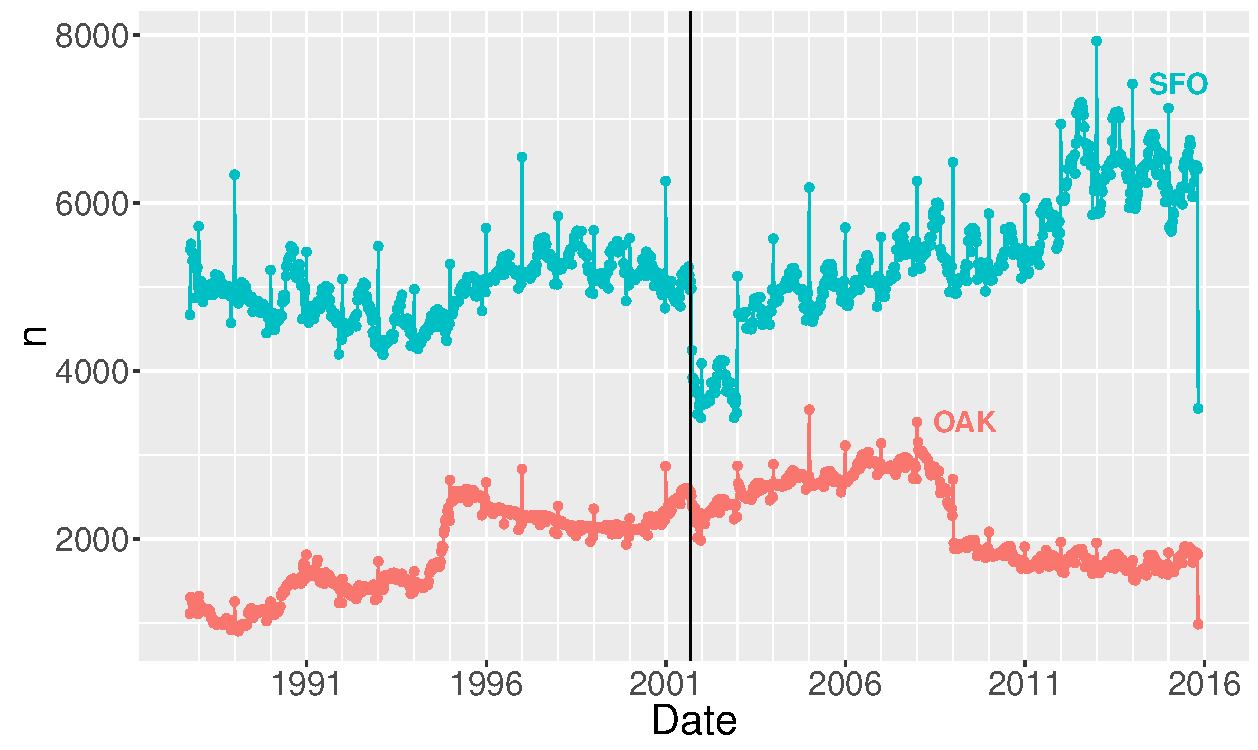
\includegraphics[width = \paperwidth]{figure/SanFran_Flights_by_date-1}}
\caption{Number of depatures over time from Oakland and San Francisco Intl.}
\end{figure}

\begin{knitrout}
\definecolor{shadecolor}{rgb}{0.969, 0.969, 0.969}\color{fgcolor}\begin{kframe}
\begin{alltt}
\hlstd{carriers} \hlkwb{<-} \hlkwd{as.data.table}\hlstd{(airlines)}
\hlkwa{if}\hlstd{(}\hlstr{"carrier"} \hlopt \hlkwd{names}\hlstd{(carriers))}
  \hlkwd{setnames}\hlstd{(carriers,} \hlkwc{old} \hlstd{=} \hlstr{"carrier"}\hlstd{,} \hlkwc{new} \hlstd{=} \hlstr{"UniqueCarrier"}\hlstd{)}

\hlkwd{setkey}\hlstd{(carriers, UniqueCarrier)}
\hlkwd{set}\hlstd{(carriers,} \hlkwc{j} \hlstd{=} \hlnum{1L}\hlstd{,} \hlkwc{value} \hlstd{=} \hlkwd{as.character}\hlstd{(carriers[[}\hlnum{1L}\hlstd{]]))}
\hlkwd{set}\hlstd{(carriers,} \hlkwc{j} \hlstd{=} \hlnum{2L}\hlstd{,} \hlkwc{value} \hlstd{=} \hlkwd{gsub}\hlstd{(}\hlstr{"^([A-Za-z]+)\textbackslash{}\textbackslash{}s.*$"}\hlstd{,} \hlstr{"\textbackslash{}\textbackslash{}1"}\hlstd{, carriers[[}\hlnum{2L}\hlstd{]]))}

\hlstd{flightsSanFran} \hlopt
  \hlkwd{filter}\hlstd{(Origin} \hlopt \hlkwd{c}\hlstd{(}\hlstr{"SFO"}\hlstd{,} \hlstr{"OAK"}\hlstd{))} \hlopt
  \hlkwd{count}\hlstd{(Year, Month, Origin, UniqueCarrier)} \hlopt
  \hlkwd{group_by}\hlstd{(UniqueCarrier)} \hlopt
  \hlkwd{filter}\hlstd{(}\hlkwd{sum}\hlstd{(n)} \hlopt{>} \hlstd{(}\hlnum{2015} \hlopt{-} \hlnum{1987}\hlstd{)} \hlopt{*} \hlnum{12} \hlopt{*} \hlnum{30}\hlstd{)}  \hlopt
  \hlkwd{mutate}\hlstd{(}\hlkwc{Date} \hlstd{= Year} \hlopt{+} \hlstd{(Month} \hlopt{-} \hlnum{1}\hlstd{)}\hlopt{/}\hlnum{12}\hlstd{)} \hlopt
  \hlkwd{setkey}\hlstd{(UniqueCarrier)} \hlopt
  \hlkwd{merge}\hlstd{(carriers)} \hlopt
  \hlkwd{ggplot}\hlstd{(}\hlkwd{aes}\hlstd{(}\hlkwc{x} \hlstd{= Date,} \hlkwc{y} \hlstd{= n} \hlopt{*} \hlstd{sample.weight.int,} \hlkwc{color} \hlstd{= name,} \hlkwc{group} \hlstd{=} \hlkwd{interaction}\hlstd{(name,Origin)))} \hlopt{+} \hlkwd{ylab}\hlstd{(}\hlstr{"Number of departures"}\hlstd{)} \hlopt{+}
  \hlkwd{geom_smooth}\hlstd{(}\hlkwc{span} \hlstd{=} \hlnum{0.25}\hlstd{,} \hlkwc{se} \hlstd{=} \hlnum{FALSE}\hlstd{)} \hlopt{+}
  \hlkwd{geom_text}\hlstd{(}\hlkwd{aes}\hlstd{(}\hlkwc{label} \hlstd{=} \hlkwd{ifelse}\hlstd{(Date} \hlopt{==} \hlkwd{max}\hlstd{(Date),}
                               \hlstd{name,}
                               \hlnum{NA_character_}\hlstd{),}
                \hlkwc{vjust} \hlstd{=} \hlkwd{ifelse}\hlstd{(name} \hlopt{==} \hlstr{"Southwest"} \hlopt{&} \hlstd{Origin} \hlopt{==} \hlstr{"SFO"}\hlstd{,}
                                 \hlopt{-}\hlnum{0.5}\hlstd{,}
                                 \hlnum{0.5}\hlstd{)),}
            \hlkwc{nudge_x} \hlstd{=} \hlnum{0.75}\hlstd{,}
            \hlkwc{size} \hlstd{=} \hlnum{5}\hlstd{)} \hlopt{+} \hlkwd{theme}\hlstd{(}\hlkwc{legend.position} \hlstd{=} \hlstr{"none"}\hlstd{)} \hlopt{+}
  \hlkwd{annotate}\hlstd{(}\hlstr{"blank"}\hlstd{,} \hlkwc{x} \hlstd{=} \hlnum{2019}\hlstd{,} \hlkwc{y} \hlstd{=} \hlnum{0}\hlstd{)} \hlopt{+}
  \hlkwd{facet_grid}\hlstd{(Origin} \hlopt{~} \hlstd{.)} \hlopt{+}
  \hlkwd{theme}\hlstd{(}\hlkwc{text} \hlstd{=} \hlkwd{element_text}\hlstd{(}\hlkwc{size} \hlstd{=} \hlnum{16}\hlstd{))}
\end{alltt}


{\ttfamily\noindent\color{warningcolor}{\#\# Warning in simpleLoess(y, x, w, span, degree = degree, parametric = parametric, : span too small.\ \  fewer data values than degrees of freedom.}}

{\ttfamily\noindent\color{warningcolor}{\#\# Warning in simpleLoess(y, x, w, span, degree = degree, parametric = parametric, : pseudoinverse used at 2002.1}}

{\ttfamily\noindent\color{warningcolor}{\#\# Warning in simpleLoess(y, x, w, span, degree = degree, parametric = parametric, : neighborhood radius 0.17125}}

{\ttfamily\noindent\color{warningcolor}{\#\# Warning in simpleLoess(y, x, w, span, degree = degree, parametric = parametric, : reciprocal condition number\ \ 0}}

{\ttfamily\noindent\color{warningcolor}{\#\# Warning in simpleLoess(y, x, w, span, degree = degree, parametric = parametric, : There are other near singularities as well. 0.029327}}

{\ttfamily\noindent\color{warningcolor}{\#\# Warning: Removed 4579 rows containing missing values (geom\_text).}}\end{kframe}
\end{knitrout}
\begin{figure}
\centering
\makebox[\textwidth]{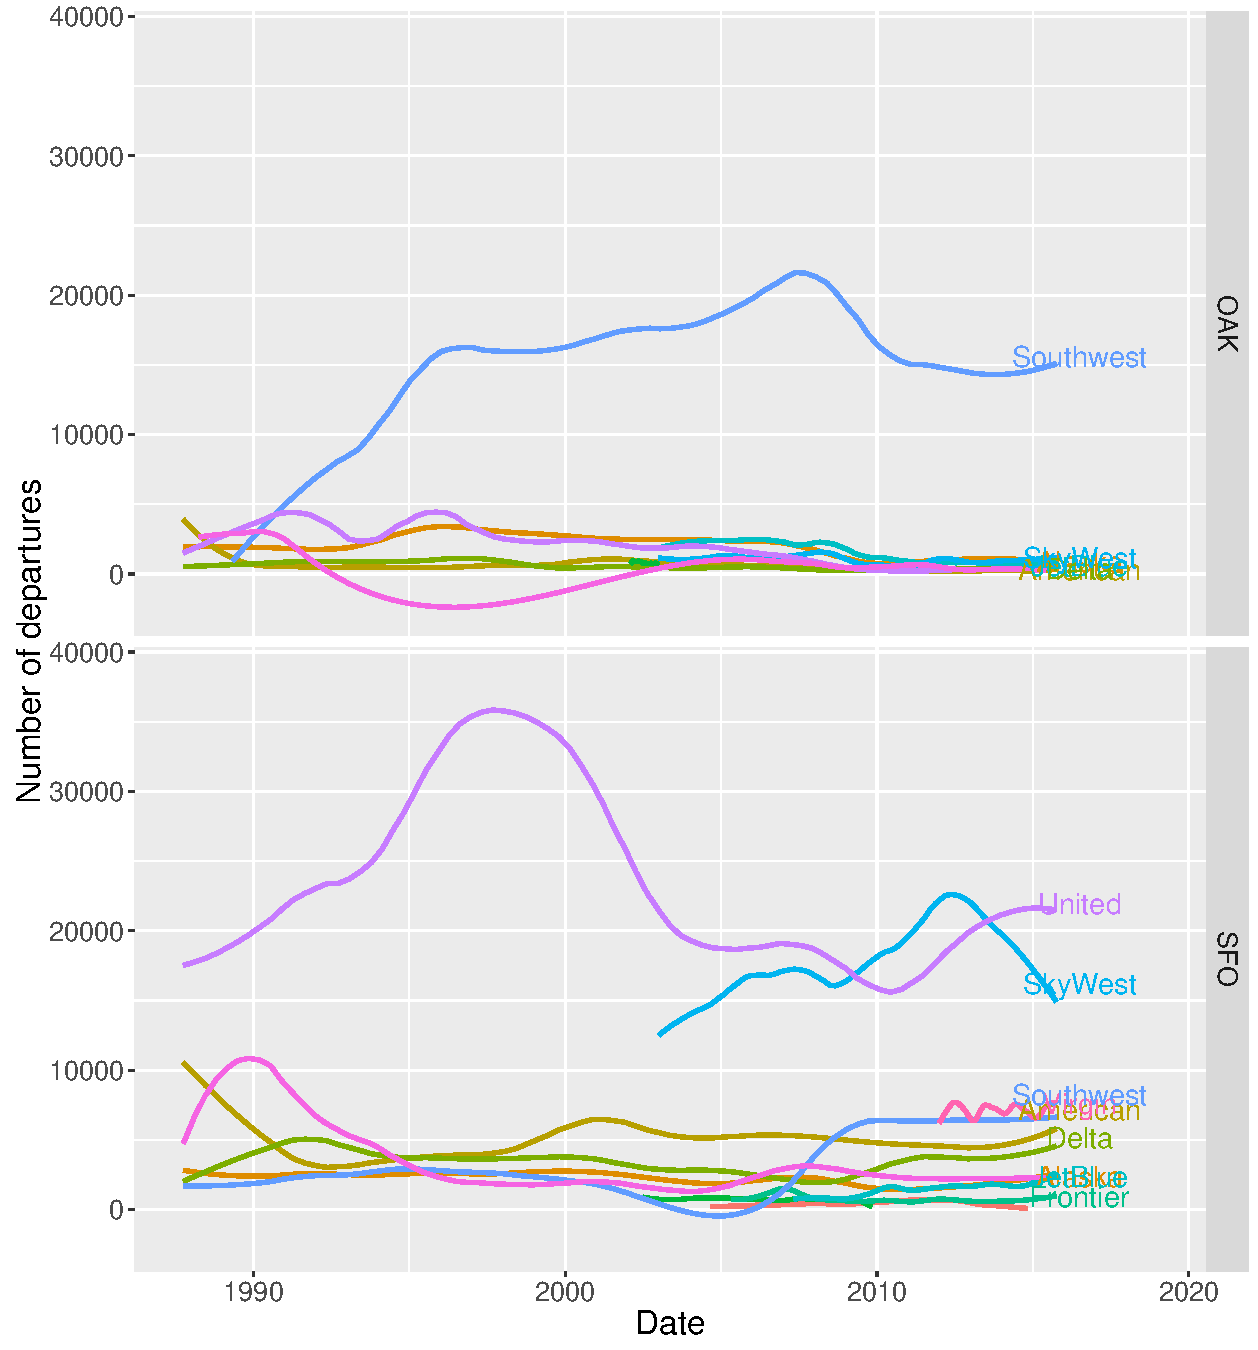
\includegraphics[width = \paperwidth]{figure/SanFran_Flights_by_Carrier-1}}
\caption{Number of depatures over time from Oakland and San Francisco Intl.}
\end{figure}

After September 11, flights from SFO fell, whereas OAK's volume did notFlights fell more in SFO than they did in OAK because most of OAK's flights are from Southwest, which did not change its flight patterns. Furthermore, United was affected more than most airlines from the aftermath of the attacks.

\begin{knitrout}
\definecolor{shadecolor}{rgb}{0.969, 0.969, 0.969}\color{fgcolor}\begin{kframe}
\begin{alltt}
\hlstd{top_5_carriers} \hlkwb{<-}
  \hlstd{flights} \hlopt
  \hlkwd{count}\hlstd{(UniqueCarrier)} \hlopt
  \hlkwd{arrange}\hlstd{(}\hlkwd{desc}\hlstd{(n))} \hlopt
  \hlkwd{mutate}\hlstd{(}\hlkwc{TopN} \hlstd{=} \hlnum{1}\hlopt{:}\hlkwd{n}\hlstd{()} \hlopt{<=} \hlnum{5}\hlstd{)} \hlopt
  \hlkwd{mutate}\hlstd{(}\hlkwc{Carrier_other} \hlstd{=} \hlkwd{ifelse}\hlstd{(TopN, UniqueCarrier,} \hlstr{"Other"}\hlstd{))} \hlopt
  \hlkwd{select}\hlstd{(}\hlopt{-}\hlstd{n)} \hlopt
  \hlkwd{setkey}\hlstd{(UniqueCarrier)}

\hlstd{flights} \hlopt
  \hlkwd{setkey}\hlstd{(UniqueCarrier)} \hlopt
  \hlkwd{merge}\hlstd{(top_5_carriers)} \hlopt
  \hlkwd{count}\hlstd{(Carrier_other, Year)} \hlopt
  \hlkwd{ggplot}\hlstd{(}\hlkwd{aes}\hlstd{(}\hlkwc{x} \hlstd{= Year,} \hlkwc{y} \hlstd{= n} \hlopt{*} \hlstd{sample.weight.int,} \hlkwc{color} \hlstd{= Carrier_other,} \hlkwc{group} \hlstd{= Carrier_other))} \hlopt{+}
  \hlkwd{geom_line}\hlstd{()} \hlopt{+}
  \hlkwd{scale_colour_brewer}\hlstd{(}\hlkwc{palette} \hlstd{=} \hlstr{"Accent"}\hlstd{)} \hlopt{+}
  \hlkwd{scale_y_continuous}\hlstd{(}\hlkwc{label} \hlstd{= scales}\hlopt{::}\hlstd{comma)}
\end{alltt}
\end{kframe}
\end{knitrout}
\begin{figure}
\makebox[\textwidth]{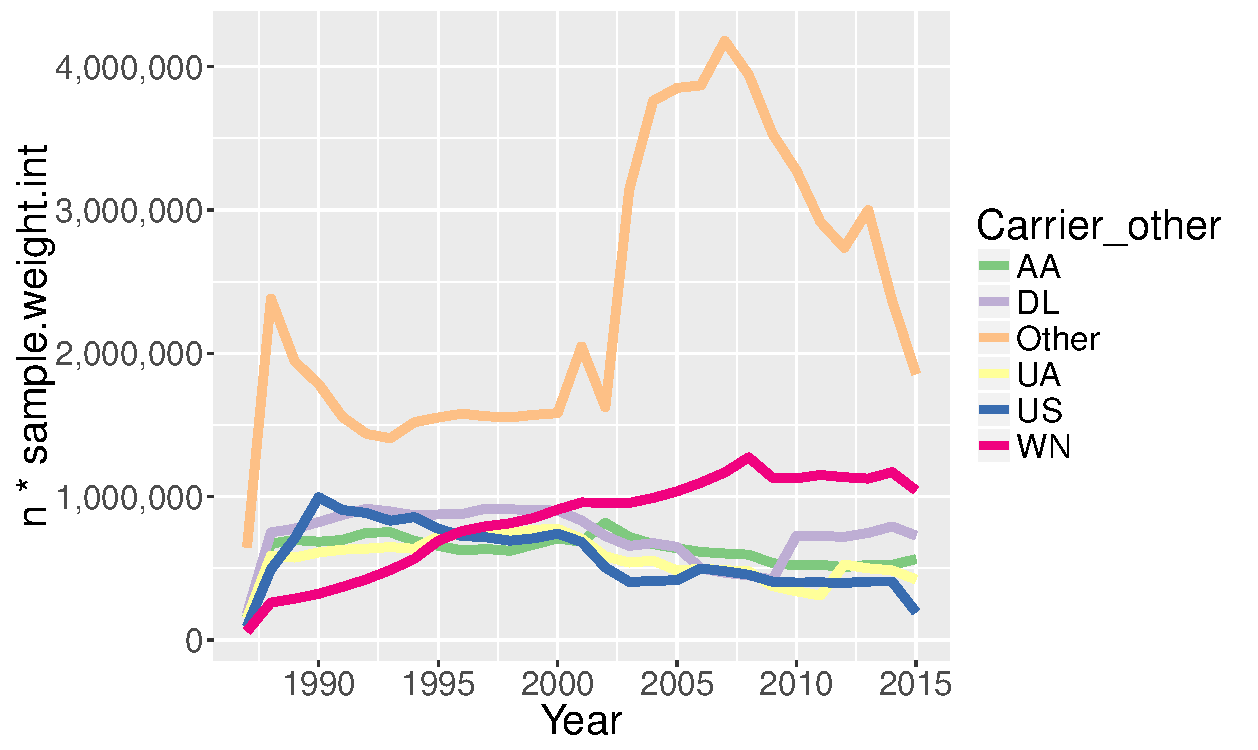
\includegraphics[width=\paperwidth]{figure/Volume-by-Carrier-1}}
\end{figure}

\begin{knitrout}
\definecolor{shadecolor}{rgb}{0.969, 0.969, 0.969}\color{fgcolor}\begin{kframe}
\begin{alltt}
\hlstd{majorAirportThreshold} \hlkwb{=} \hlnum{10}

\hlstd{airports_by_volume_by_year} \hlkwb{<-} \hlstd{flights[major_airports][ ,}\hlkwd{.}\hlstd{(}\hlkwc{n} \hlstd{= .N} \hlopt{*} \hlstd{sample.weight.int),} \hlkwc{by} \hlstd{=} \hlkwd{list}\hlstd{(Year, AirportOther)]}
\end{alltt}


{\ttfamily\noindent\bfseries\color{errorcolor}{\#\# Error in eval(expr, envir, enclos): object 'major\_airports' not found}}\begin{alltt}
\hlstd{airports_by_volume_by_2014} \hlkwb{<-}
  \hlstd{airports_by_volume_by_year} \hlopt
  \hlkwd{filter}\hlstd{(Year} \hlopt{==} \hlnum{2014}\hlstd{)} \hlopt
  \hlkwd{filter}\hlstd{(AirportOther} \hlopt{!=} \hlstr{"AirportOther"}\hlstd{)} \hlopt
  \hlkwd{merge}\hlstd{(}\hlkwd{select}\hlstd{(nycflights.airports, faa, name),} \hlkwc{by.x} \hlstd{=} \hlstr{"AirportOther"}\hlstd{,} \hlkwc{by.y} \hlstd{=} \hlstr{"faa"}\hlstd{)} \hlopt
  \hlkwd{arrange}\hlstd{(}\hlkwd{desc}\hlstd{(n))}
\end{alltt}


{\ttfamily\noindent\bfseries\color{errorcolor}{\#\# Error in eval(expr, envir, enclos): object 'airports\_by\_volume\_by\_year' not found}}\begin{alltt}
\hlkwd{gc}\hlstd{(}\hlnum{0}\hlstd{,}\hlnum{1}\hlstd{)}
\end{alltt}
\begin{verbatim}
##             used   (Mb) gc trigger    (Mb)  max used   (Mb)
## Ncells    691026   37.0    2423100   129.5    691026   37.0
## Vcells 988301793 7540.2 2790305607 21288.4 988301793 7540.2
\end{verbatim}
\begin{alltt}
\hlstd{major_airports} \hlkwb{<-}
  \hlstd{flights[ ,}\hlkwd{.}\hlstd{(}\hlkwc{n} \hlstd{= .N),} \hlkwc{by} \hlstd{= Dest][}\hlkwd{order}\hlstd{(}\hlopt{-}\hlstd{n)]} \hlopt \hlcom{# flights %>% count(Dest) %>% arrange(desc(n))}
  \hlkwd{mutate}\hlstd{(}\hlkwc{TopN} \hlstd{=} \hlnum{1}\hlopt{:}\hlkwd{n}\hlstd{()} \hlopt{<=} \hlstd{majorAirportThreshold)} \hlopt
  \hlkwd{mutate}\hlstd{(}\hlkwc{AirportOther} \hlstd{=} \hlkwd{ifelse}\hlstd{(TopN, Dest,} \hlstr{"Other_airport"}\hlstd{))} \hlopt
  \hlkwd{select}\hlstd{(}\hlopt{-}\hlstd{n)} \hlopt
  \hlkwd{setkey}\hlstd{(Dest)}
\hlkwd{setkey}\hlstd{(flights, Dest)}
\hlkwd{gc}\hlstd{(}\hlnum{0}\hlstd{,}\hlnum{1}\hlstd{)}
\end{alltt}
\begin{verbatim}
##             used   (Mb) gc trigger    (Mb)  max used   (Mb)
## Ncells    691069   37.0    2423100   129.5    691069   37.0
## Vcells 988303478 7540.2 2790305607 21288.4 988303478 7540.2
\end{verbatim}
\begin{alltt}
\hlstd{airports_by_volume_by_year} \hlopt
  \hlkwd{filter}\hlstd{(AirportOther} \hlopt{!=} \hlstr{"Other_airport"}\hlstd{, Year} \hlopt{>} \hlnum{1987L}\hlstd{, Year} \hlopt{<} \hlnum{2015L}\hlstd{)}  \hlopt
  \hlkwd{merge}\hlstd{(}\hlkwd{select}\hlstd{(nycflights.airports, faa, name),} \hlkwc{by.x} \hlstd{=} \hlstr{"AirportOther"}\hlstd{,} \hlkwc{by.y} \hlstd{=} \hlstr{"faa"}\hlstd{)} \hlopt
  \hlkwd{mutate}\hlstd{(}\hlkwc{name} \hlstd{=} \hlkwd{factor}\hlstd{(name,} \hlkwc{levels} \hlstd{= airports_by_volume_by_2014}\hlopt{$}\hlstd{name))} \hlopt
  \hlkwd{ggplot}\hlstd{(}\hlkwd{aes}\hlstd{(}\hlkwc{x} \hlstd{= Year,} \hlkwc{y} \hlstd{= n,} \hlkwc{group} \hlstd{= name,} \hlkwc{color} \hlstd{= name))} \hlopt{+}
  \hlkwd{geom_line}\hlstd{()}
\end{alltt}


{\ttfamily\noindent\bfseries\color{errorcolor}{\#\# Error in eval(expr, envir, enclos): object 'airports\_by\_volume\_by\_year' not found}}\begin{alltt}
\hlkwd{gc}\hlstd{(}\hlnum{0}\hlstd{,}\hlnum{1}\hlstd{)}
\end{alltt}
\begin{verbatim}
##             used   (Mb) gc trigger    (Mb)  max used   (Mb)
## Ncells    691045   37.0    2423100   129.5    691045   37.0
## Vcells 988301906 7540.2 2790305607 21288.4 988301906 7540.2
\end{verbatim}
\end{kframe}
\end{knitrout}

\begin{knitrout}
\definecolor{shadecolor}{rgb}{0.969, 0.969, 0.969}\color{fgcolor}\begin{kframe}
\begin{alltt}
\hlstd{rel_vol_major_airports} \hlkwb{<-}
  \hlstd{flights[major_airports][ ,}\hlkwd{.}\hlstd{(}\hlkwc{n} \hlstd{= .N} \hlopt{*} \hlstd{sample.weight.int),} \hlkwc{by} \hlstd{=} \hlkwd{list}\hlstd{(Year, AirportOther)]} \hlopt
  \hlkwd{filter}\hlstd{(AirportOther} \hlopt{!=} \hlstr{"Other_airport"}\hlstd{, Year} \hlopt{>} \hlnum{1987L}\hlstd{, Year} \hlopt{<} \hlnum{2015L}\hlstd{)} \hlopt
  \hlkwd{arrange}\hlstd{(Year)} \hlopt
  \hlkwd{group_by}\hlstd{(AirportOther)} \hlopt
  \hlkwd{mutate}\hlstd{(}\hlkwc{rel} \hlstd{= n}\hlopt{/}\hlkwd{first}\hlstd{(n))} \hlopt
  \hlkwd{merge}\hlstd{(}\hlkwd{select}\hlstd{(nycflights.airports, faa, name),} \hlkwc{by.x} \hlstd{=} \hlstr{"AirportOther"}\hlstd{,} \hlkwc{by.y} \hlstd{=} \hlstr{"faa"}\hlstd{)}

\hlstd{last_values} \hlkwb{<-}
  \hlstd{rel_vol_major_airports} \hlopt
  \hlkwd{filter}\hlstd{(Year} \hlopt{==} \hlkwd{max}\hlstd{(Year))} \hlopt
  \hlkwd{arrange}\hlstd{(rel)}

\hlstd{otp201510} \hlkwb{<-}
  \hlkwd{fread}\hlstd{(}\hlstr{"../dep_delay/On_Time_On_Time_Performance_2015_10.csv"}\hlstd{)}
\end{alltt}
\begin{verbatim}
## 
Read 57.6% of 486165 rows
Read 92.6% of 486165 rows
Read 486165 rows and 110 (of 110) columns from 0.204 GB file in 00:00:04
\end{verbatim}
\begin{alltt}
\hlstd{otp201510} \hlopt
  \hlkwd{select}\hlstd{(}\hlkwd{contains}\hlstd{(}\hlstr{"Origin"}\hlstd{))}
\end{alltt}
\begin{verbatim}
##         OriginAirportID OriginAirportSeqID OriginCityMarketID Origin
##      1:           12478            1247803              31703    JFK
##      2:           12478            1247803              31703    JFK
##      3:           12478            1247803              31703    JFK
##      4:           12478            1247803              31703    JFK
##      5:           12478            1247803              31703    JFK
##     ---                                                             
## 486161:           13830            1383002              33830    OGG
## 486162:           13830            1383002              33830    OGG
## 486163:           13830            1383002              33830    OGG
## 486164:           13830            1383002              33830    OGG
## 486165:           12173            1217302              32134    HNL
##         OriginCityName OriginState OriginStateFips OriginStateName
##      1:   New York, NY          NY              36        New York
##      2:   New York, NY          NY              36        New York
##      3:   New York, NY          NY              36        New York
##      4:   New York, NY          NY              36        New York
##      5:   New York, NY          NY              36        New York
##     ---                                                           
## 486161:    Kahului, HI          HI              15          Hawaii
## 486162:    Kahului, HI          HI              15          Hawaii
## 486163:    Kahului, HI          HI              15          Hawaii
## 486164:    Kahului, HI          HI              15          Hawaii
## 486165:   Honolulu, HI          HI              15          Hawaii
##         OriginWac
##      1:        22
##      2:        22
##      3:        22
##      4:        22
##      5:        22
##     ---          
## 486161:         2
## 486162:         2
## 486163:         2
## 486164:         2
## 486165:         2
\end{verbatim}
\begin{alltt}
\hlstd{rel_vol_major_airports}  \hlopt
  \hlkwd{mutate}\hlstd{(}\hlkwc{name} \hlstd{=} \hlkwd{factor}\hlstd{(name,} \hlkwc{levels} \hlstd{=} \hlkwd{rev}\hlstd{(last_values}\hlopt{$}\hlstd{name)))} \hlopt
  \hlkwd{ggplot}\hlstd{(}\hlkwd{aes}\hlstd{(}\hlkwc{x} \hlstd{= Year,} \hlkwc{y} \hlstd{= rel,} \hlkwc{group} \hlstd{= name,} \hlkwc{color} \hlstd{= name))} \hlopt{+}
  \hlkwd{geom_line}\hlstd{()}
\end{alltt}
\end{kframe}
\end{knitrout}
\begin{figure}
\makebox[\textwidth]{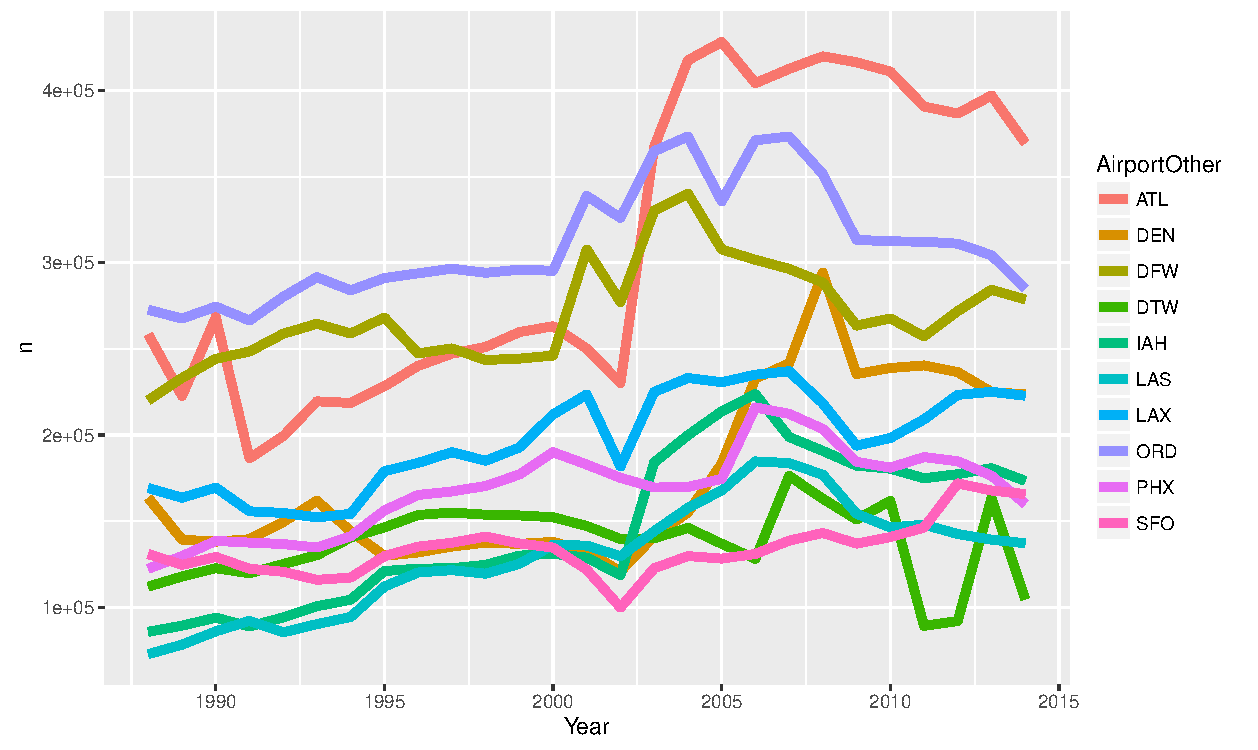
\includegraphics[width=\paperwidth]{figure/Volume-by-major-airports-1}}
\caption{Annual flights by the top 10 airports by total volume.}
\end{figure}

\begin{figure}
\makebox[\textwidth]{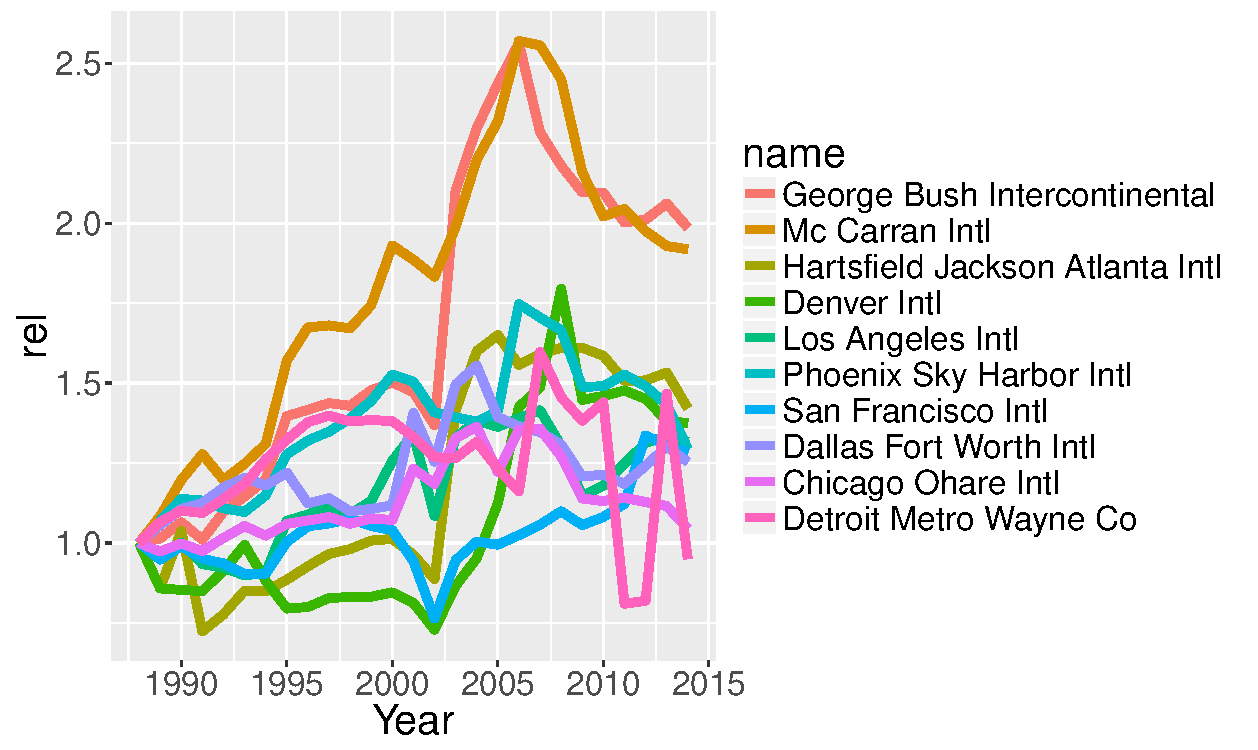
\includegraphics[width=\paperwidth]{figure/Relative-volume-by-major-airports-1}}
\caption{Annual flights by airport, 1988 = 1.}
\end{figure}


\begin{knitrout}
\definecolor{shadecolor}{rgb}{0.969, 0.969, 0.969}\color{fgcolor}\begin{kframe}
\begin{alltt}
\hlstd{FINISH.TIME} \hlkwb{<-} \hlkwd{Sys.time}\hlstd{()}
\end{alltt}
\end{kframe}
\end{knitrout}
Compiled in 12.2163051843643
\end{document}
